\documentclass[a4paper,
fontsize=11pt,
%headings=small,
oneside,
numbers=noperiodatend,
parskip=half-,
bibliography=totoc,
final
]{scrartcl}

\usepackage{synttree}
\usepackage{graphicx}
\setkeys{Gin}{width=.4\textwidth} %default pics size

\graphicspath{{./plots/}}
\usepackage[ngerman]{babel}
\usepackage[T1]{fontenc}
%\usepackage{amsmath}
\usepackage[utf8x]{inputenc}
\usepackage [hyphens]{url}
\usepackage{booktabs} 
\usepackage[left=2.4cm,right=2.4cm,top=2.3cm,bottom=2cm,includeheadfoot]{geometry}
\usepackage{eurosym}
\usepackage{multirow}
\usepackage[ngerman]{varioref}
\setcapindent{1em}
\renewcommand{\labelitemi}{--}
\usepackage{paralist}
\usepackage{pdfpages}
\usepackage{lscape}
\usepackage{float}
\usepackage{acronym}
\usepackage{eurosym}
\usepackage[babel]{csquotes}
\usepackage{longtable,lscape}
\usepackage{mathpazo}
\usepackage[normalem]{ulem} %emphasize weiterhin kursiv
\usepackage[flushmargin,ragged]{footmisc} % left align footnote
\usepackage{ccicons} 
\setcapindent{0pt} % no indentation in captions

%%%% fancy LIBREAS URL color 
\usepackage{xcolor}
\definecolor{libreas}{RGB}{112,0,0}

\usepackage{listings}

\urlstyle{same}  % don't use monospace font for urls

\usepackage[fleqn]{amsmath}

%adjust fontsize for part

\usepackage{sectsty}
\partfont{\large}

%Das BibTeX-Zeichen mit \BibTeX setzen:
\def\symbol#1{\char #1\relax}
\def\bsl{{\tt\symbol{'134}}}
\def\BibTeX{{\rm B\kern-.05em{\sc i\kern-.025em b}\kern-.08em
    T\kern-.1667em\lower.7ex\hbox{E}\kern-.125emX}}

\usepackage{fancyhdr}
\fancyhf{}
\pagestyle{fancyplain}
\fancyhead[R]{\thepage}

% make sure bookmarks are created eventough sections are not numbered!
% uncommend if sections are numbered (bookmarks created by default)
%\makeatletter
%\renewcommand\@seccntformat[1]{}
%\makeatother

% typo setup
\clubpenalty = 10000
\widowpenalty = 10000
\displaywidowpenalty = 10000

\usepackage{hyperxmp}
\usepackage[colorlinks, linkcolor=black,citecolor=black, urlcolor=libreas,
breaklinks= true,bookmarks=true,bookmarksopen=true]{hyperref}
\usepackage{breakurl}

%meta
%meta

\fancyhead[L]{K. Schuldt\\ %author
LIBREAS. Library Ideas, 35 (2019). % journal, issue, volume.
\href{http://nbn-resolving.de/}
{}} % urn 
% recommended use
%\href{http://nbn-resolving.de/}{\color{black}{urn:nbn:de...}}
\fancyhead[R]{\thepage} %page number
\fancyfoot[L] {\ccLogo \ccAttribution\ \href{https://creativecommons.org/licenses/by/4.0/}{\color{black}Creative Commons BY 4.0}}  %licence
\fancyfoot[R] {ISSN: 1860-7950}

\title{\LARGE{Neutralität als bürgerliche Bibliotheksideologie. Die Kritik der \enquote{Arbeiterbibliotheken} zu Beginn des 20. Jahrhunderts}}% title
\author{Karsten Schuldt} % author

\setcounter{page}{1}

\hypersetup{%
      pdftitle={Neutralität als bürgerliche Bibliotheksideologie. Die Kritik der "Arbeiterbibliotheken" zu Beginn des 20. Jahrhunderts},
      pdfauthor={Karsten Schuldt},
      pdfcopyright={CC BY 4.0 International},
      pdfsubject={LIBREAS. Library Ideas, 35 (2019).},
      pdfkeywords={Bibliotheksgeschichte, Arbeiterbewegung, Deutschland, Österreich, Bestandsaufbau, sozialistische Bewegung},
      pdflicenseurl={https://creativecommons.org/licenses/by/4.0/},
      pdfcontacturl={http://libreas.eu},
      baseurl={http://libreas.eu},
      pdflang={de},
      pdfmetalang={de}
     }



\date{}
\begin{document}

\maketitle
\thispagestyle{fancyplain} 

%abstracts

%body
\hypertarget{einleitung}{%
\section{Einleitung}\label{einleitung}}

Dass Bibliotheken bei Bestandsaufbau und -vermittlung die inhaltliche
Neutralität als Leitbild haben, ist Ausdruck eines konkreten Weltbildes.
Nur aus einem spezifischen Verständnis davon, wie Gesellschaft
funktioniert, lässt sich \enquote{Neutralität} als anzustrebendes Ziel
als praktisch unhinterfragbar positiv werten oder gar behaupten, dass
Bibliotheken tatsächlich neutrale Räume und Institutionen wären (also
das Ziel und Realität in eins fallen würden).

Dieses Weltbild soll in diesem Text allerdings nicht direkt untersucht,
also keine Ideologiekritik betrieben werden. Das wäre ein zu komplexes
Unternehmen, schon weil es notwendig wäre, die Veränderungen desselben
über die Jahrzehnte nachzuzeichnen. Es soll hier auch keine inhaltliche
Kritik des Weltbilds unternommen werden. Was in diesem Text stattdessen
versucht wird, ist anhand der Geschichte eines heute verschwundenen
Bibliothekstyps -- dem der \enquote{Arbeiterbibliotheken}\footnote{Der
  Begriff \enquote{Arbeiterbibliotheken} wurde zeitgenössisch von den
  Bibliotheken der \enquote{Arbeiterbewegung} selber und auch von
  anderen Bibliotheken und Bewegungen für diesen Bibliothekstyp benutzt.
  Obgleich die \enquote{Arbeiterbewegung} auch für Frauenrechte wie das
  Frauenwahlrecht, für die Aufhebung von Abtreibungsverboten und für die
  Aufklärung über Abtreibungen und Geburt eintrat, war ihre Sprache
  teilweise ausschliessend. Arbeiterinnen wurden damals tatsächlich
  \enquote{mitgemeint}. Der Autor würde heute eine inklusivere
  Bezeichnung wählen -- zum Beispiel ArbeiterInnenbibliothek,
  proletarische Bibliothek --, das wäre aber anachronistisch. Deshalb
  wird die Bezeichnung im Text in Anführungszeichen gesetzt. Gleiches
  gilt für die \enquote{Arbeiterbewegung} selber.} -- vom Ende des 19.
und Anfang des 20. Jahrhunderts in Deutschland und Österreich zu zeigen,
dass die Grundidee, eine Öffentliche Bibliothek müsse neutral sein im
Bezug auf Zugang, Angebot, Vermittlung und Bestand, nicht alternativlos
ist. Lange existierten Bibliotheken, die dies explizit nicht waren, die
zugleich ihre Abgrenzung zu \enquote{neutralen} Bibliotheken begründeten
und die zudem erfolgreich arbeiteten. Wenn die heute propagierte Form
von Öffentlichen Bibliotheken aber nicht alternativlos ist, dann lässt
sich sinnvoll fragen, wieso sie dann heute so ist, wie sie ist oder sein
soll, wie sie sein soll. Geschichte macht hier das Nachdenken über die
Aufgaben und Möglichkeiten von Bibliotheken komplexer.

Der Text ist wie folgt aufgebaut: Zuerst wird kurz die Geschichte der
\enquote{Arbeiterbibliotheken} geschildert. (2) Dazu ist es notwendig,
den Kontext -- also die sozialistische Bewegung und die
gesellschaftlichen Auseinandersetzungen der damaligen Zeit -- zu
skizzieren. Anschliessend wird die Argumentation der Bibliotheken für
ihre eigene Existenz und für ihre Abgrenzung von anderen
Bibliothekstypen, insbesondere den Lesehallen, und ihre Kritik an diesen
dargelegt. (3) Interessant ist -- wie geschildert werden wird --, dass
die \enquote{Arbeiterbibliotheken} trotz ihrer Kritik grundlegende
Überzeugungen mit den von ihnen kritisierten \enquote{bürgerlichen
Bibliotheken} (und weiteren Bibliothekstypen) teilten. Vor dem Fazit
wird das Ende der \enquote{Arbeiterbibliotheken} besprochen, da anders
die Frage, ob ihre Kritik weiterhin berechtigt ist oder als erledigt
gelten kann, nicht fair anzugehen wäre. (4) Auf dieser Basis wird im
Fazit diskutiert, ob das Beispiel der Kritik der
\enquote{Arbeiterbibliotheken} auch etwas über die Weltanschauung sagt,
aus der heraus heute die \enquote{Neutralität} von Bibliotheken als
anzustrebendes Ziel hergeleitet wird, oder ob sie ein rein historischer
Fakt ist. (5)

\hypertarget{was-waren-arbeiterbibliotheken-ein-kurzer-uxfcberblick}{%
\section{\texorpdfstring{Was waren \enquote{Arbeiterbibliotheken}?
Ein kurzer
Überblick}{Was waren \enquote{Arbeiterbibliotheken}? Ein kurzer Überblick}}\label{was-waren-arbeiterbibliotheken-ein-kurzer-uxfcberblick}}

Die Kritik an den \enquote{bürgerlichen Bibliotheken} -- den
Volksbüchereien, den Lesehallen und ähnlichen kommunal oder durch
Philanthropie getragenen Bibliotheken --, die aus den
\enquote{Arbeiterbibliotheken} heraus formuliert wurde, ist nur
verständlich aus der Arbeit dieser Einrichtungen selber. Diese Arbeit
benötigt wiederum eine historische Kontextualisierung. Deshalb wird in
diesem Kapitel zuerst als Hintergrund die \enquote{Arbeiterbewegung}
Ende des 19. und Anfang des 20. Jahrhunderts geschildert (2.1),
anschliessend die Arbeit der Bibliotheken dieser Bewegung (2.2) und ihre
Bestandsarbeit (2.3).

\hypertarget{die-damalige-sozialistische-bewegung-in-deutschland-und-uxf6sterreich}{%
\subsection{Die damalige sozialistische Bewegung in Deutschland und
Österreich}\label{die-damalige-sozialistische-bewegung-in-deutschland-und-uxf6sterreich}}

Die Industrialisierung in Deutschland und Österreich ging bekanntlich
einher mit dem Entstehen der \enquote{Arbeiterbewegung} mit all ihren
Spielarten, Strömungen und Institutionen.\footnote{In diesem Text geht
  es um die \enquote{Arbeiterbibliotheken} seit den 1880er Jahren. Die
  \enquote{Arbeiterbildungsvereine} um 1848 unterhielten ebenso
  Bibliotheken (siehe zu diesen Brünle 2010), aber ebenso wie die
  \enquote{Arbeiter} von 1848 schwerlich mit den späteren
  Fabrikarbeiterinnen und -arbeitern zu vergleichen sind, sind es auch
  deren Bibliotheken.} Durch das Entstehen einer ausreichend grossen
Schicht von Industriearbeiterinnen und -arbeitern und ihrer
Selbstorganisation in Gruppierungen, Gewerkschaften und Parteien wurde
diese zu einem relevanten politischen Faktor. Von anderen Schichten und
Bewegungen wurden sie in der Folge als Gefahr angesehen, gegen die
vorzugehen sei, was wiederum die innere Konsistenz der Bewegung
verstärkte. Die \enquote{Sozialistengesetze}, welche von 1878 bis 1890
im Deutschen Reich in Kraft waren, sind nur der heute bekannteste
Ausdruck dieser Entwicklung.

Die Strömungen der \enquote{Arbeiterbewegung} einte damals das Ziel,
eine gänzlich anders organisierte Gesellschaft anzustreben. Diese wurde
sehr unterschiedlich bezeichnet -- Sozialismus, Kommunismus, Anarchismus
und so weiter --, und unterschiedlich imaginiert -- ohne Staat und mit
allgemeiner Selbstorganisation; mit \enquote{absterbendem Staat}, der
sich langsam selbst aufheben sollte und anders. Zum Erreichen dieses
Ziels wurden schließlich unterschiedliche Wege -- revolutionäre
Erhebung, Übernahme der Staatsmacht, religiöse oder quasi-religiöse
Erweckung, langsame Eroberung der politischen Macht, Aufbau von
Strukturen und Institutionen, die letztlich die alten Strukturen
ersetzen sollten -- vorgeschlagen und erprobt. Zumindest die Teile der
Bewegung, welche sich als theoretische Grundlage auf die Arbeiten von
Karl Marx und Friedrich Engels beriefen, gingen dabei einerseits davon
aus, dass die ökonomische Struktur des Kapitalismus zu unterschiedlichen
Klassen führt, welche gesellschaftlich produziert sind, und andererseits
davon, dass diese Klassen gegeneinander im Widerstreit stehen, da sie
unterschiedliche ökonomische Interessen hätten, die innerhalb der
existierenden Gesellschaft nicht aufzulösen wären, sondern immer wieder
reproduziert würden. Auf der Basis dieses \enquote{antagonistischen
Widerspruchs} wurden andere -- wahrgenommene -- Unterschiede innerhalb
der Gesellschaft etabliert.

Auch wenn diese Bewegung heute -- lange nach dem Zusammenbruch des
\enquote{real-existierenden Sozialismus} -- in der allgemeinen
Erinnerung kaum noch vorhanden zu sein scheint, war sie ab der zweiten
Hälfte des 19. Jahrhunderts eine dynamische, aktive, breitenwirksame
Bewegung, bei der lange zu vermuten war, dass sie ihr grundlegendes Ziel
-- die sozialistische Gesellschaft in einer ihrer angestrebten Formen --
im Laufe der Zeit erringen könnte.

Aus dieser Bewegung heraus wurde kontinuierlich Kritik an der
bestehenden Gesellschaft geübt. Nicht nur an den ökonomischen
Verhältnissen, welche ja die Basis der Bewegung bildeten, sondern auch
an den staatlichen, juristischen, kulturellen und anderen Strukturen. Zu
dieser Kritik gehörte selbstverständlich auch, sich darüber Gedanken zu
machen, wie diese gesellschaftlichen Strukturen wirkten. Letztlich, so
eine schwer zurückzuweisende Grundthese, waren die vorhandenen
Strukturen dafür verantwortlich, dass die Gesellschaft so war und
funktionierte, wie sie es tat. Das hiess nicht unbedingt, dass alles
Bestehende vollständig abgelehnt wurde, aber oft hiess es, dass gefragt
wurde, wie etwas Existierendes für die \enquote{Arbeiterbewegung} und
für die zukünftige Gesellschaft übernommen, verändert und genutzt werden
könnte -- und wie es gleichzeitig in seiner bisherigen Verfasstheit dazu
beiträgt, die als falsch angesehene Gesellschaft zu reproduzieren. Diese
Kritik und Überlegungen bezogen sich auch auf Öffentliche Bibliotheken
(beziehungsweise, in der damaligen Terminologie, Büchereien und -- wie
weiter unten (3) gezeigt wird -- Lesehallen).

Die \enquote{Arbeiterbewegung} baute Vereine, Strukturen, Institutionen
auf, die weit über Parteien und Gewerkschaften hinaus gingen. Es wurden
umfassende Subkulturen geschaffen, in denen Personen ihren gesamten
Alltag, neben der Arbeit selber, organisieren konnten: Produktions- und
Einkaufsgenossenschaften, Gesangs- und Sportvereine, Heime, Kneipen,
Versicherungen, Publikationsorgane und Verlage, Theater, Ferienlager und
vieles mehr. Nur dort, wo der Staat sich die explizite Kontrolle
zusprach und durchsetzte -- wie der Organisation der Schule oder, im
\enquote{Kulturkampf} gegen den politisch organisierten Katholizismus,
bei der Eheschliessung -- konnte die Arbeiterbewegung keinen Ersatz
bereitstellen. Aber auch in diesen Bereichen wurde versucht, den
staatlichen Einfluss durch Zusatzangebote zurückzudrängen, zum Beispiel
einem eigenen, ergänzenden Bildungssystem. Dies war keine Eigenheit der
\enquote{Arbeiterbewegung}. Praktisch alle politischen Bewegungen bis
zur Mitte des 20. Jahrhunderts tendierten dazu, solche
\enquote{Partikularkulturen} zu etablieren, wobei einige erfolgreicher
waren als andere, insbesondere bezogen auf eine Massenbasis. Die
\enquote{Arbeiterbewegung} war hierbei extrem erfolgreich, ebenso für
lange Zeit der schon genannte politisch organisierte Katholizismus --
nicht zufällig die beiden Bewegungen, gegen die im Deutschen Reich
politisch vorgegangen wurde. Jede Ausdifferenzierung oder gesonderte
Strömung, welche innerhalb der \enquote{Arbeiterbewegung} entstand,
tendierte dazu, eine eigene Partikularkultur entweder zu etablieren oder
von der jeweiligen Strömung, aus der sie hervorgegangen waren, zu
übernehmen.\footnote{So dass irgendwann in grösseren Städten
  sozialdemokratische, kommunistische, anarchistische,
  anarcho-syndikalistische, räte-kommunistische und weitere Heime,
  Kneipen, Jugendorganisationen und Sportvereine nebeneinander
  existieren konnten, ebenso wie deren Parteien, politische
  Organisationen und Gewerkschaften, die allesamt zur
  \enquote{Arbeiterbewegung} gezählt wurden -- auch wenn sie alle ihre
  politischen Differenzen hatten. Die \enquote{Arbeiterbibliotheken}, um
  die es in diesem Text geht, waren zumeist solche der
  \enquote{Mehrheitströmung}, die bei der SPD respektive SPÖ verblieben.
  Es wäre aber selbstverständlich interessant, auch in der
  Bibliotheksgeschichte den Verzweigungen und Spaltungen der
  \enquote{Arbeiterbewegung} nachzugehen.} Auch dies machte vor den
Bibliotheken nicht halt. Die \enquote{Arbeiterbibliotheken}, um die es
hier gehen soll, müssen vor diesem Hintergrund gesehen werden.

\hypertarget{arbeiterbibliotheken}{%
\subsection{\texorpdfstring{\enquote{Arbeiterbibliotheken}}{\enquote{Arbeiterbibliotheken}}}\label{arbeiterbibliotheken}}

\enquote{Arbeiterbibliotheken} waren Bibliotheken, die aus der
\enquote{Arbeiterbewegung} heraus für Mitglieder dieser Bewegung
gegründet wurde. Sie wuchsen mit der Bewegung selber und erreichten in
einigen Regionen und Orten eine Professionalität, die mindestens
vergleichbar war mit anderen Büchereien und Lesehallen. Dies war nicht
überall der Fall, aber diese regionalen Unterschiede galten nicht nur
für \enquote{Arbeiterbibliotheken}. Die Regionen, über welche heute noch
die meisten Informationen über \enquote{Arbeiterbibliotheken} vorliegen,
waren nicht zufällig solche, in denen die \enquote{Arbeiterbewegung} und
die Industrialisierung stark waren: Das Sächsisch-Thüringische
Industriegebiet, Wien und der Berlin-Brandenburgische Raum.\footnote{Forschung
  zu \enquote{Arbeiterbibliotheken} wird nicht systematisch betrieben
  (dazu auch schon Vodosek 1975). Mit \enquote{Der Bibliothekar}
  (1907--1922, Leipzig und Gera), herausgegeben von Gustav Hennig, und
  der \enquote{Bildungsarbeit. Blätter für Sozialistisches
  Bildungswesen} (1909--1914 und 1919--1934, Wien), herausgegeben von
  der SPÖ, liegen zwei zeitgenössische Zeitschriften -- letztere auch
  digitalisiert -- mit einem Fokus auf \enquote{Arbeiterbibliotheken}
  als Quellen vor. Zudem Material von und zu Gustav Hennig selber
  (Hennig 1908, Marwinski 1994), zu \enquote{Arbeiterbibliotheken} in
  Thüringen -- die zum Teil auch von Hennig beraten wurden -- (Schroeder
  2008), zu den Arbeiterbibliotheken im Austromarxismus (Pfoser 1980,
  Heidenreich 1995) und zur \enquote{Heimannschen Bibliothek} in Berlin
  (Stroscher 1987). Es gab aber auch weitere, eher kurzlebige
  Zeitschriften, zudem Erwähnungen in der Presse der
  \enquote{Arbeiterbewegung} oder Diskussionen auf Kongressen,
  Tagesordnungspunkte bei Partei- und Gewerkschaftstreffen und so
  weiter. Gerade für die Zentren der damaligen
  \enquote{Arbeiterbewegung} -- zum Beispiel Hamburg, das Rheinland,
  Zürich, Basel oder Genf -- wäre zu erwarten, dass eine systematische
  Forschung weit mehr zur Geschichte der \enquote{Arbeiterbibliotheken}
  an den Tag bringen würde.}

Die \enquote{Arbeiterbibliotheken} entwickelten sich mit der
\enquote{Arbeiterbewegung} und wurden von dieser getragen. Das heisst
auch, dass die Räume, Bestände, das -- meist ehrenamtliche -- Personal
und der Etat von der \enquote{Arbeiterbewegung} gestellt und finanziert
wurden, jeweils lokal von den örtlichen Parteisektionen, Gewerkschaften
und anderen Vereinen. Zur Zeit der \enquote{Sozialistengesetze} -- als
Aktivitäten von sozialdemokratischen oder ähnlichen Vereinen oder gar
Parteien und Gewerkschaften, die über den lokalen Rahmen hinausgingen,
bekanntlich verboten waren -- wurden auch die Bibliotheken lokal
organisiert. Nachdem die \enquote{Arbeiterbewegung} trotz dieser Gesetze
weiter gewachsen war und diese nicht mehr verlängert wurden, etablierte
sich die Bewegung mit eigenen Parteizentralen, Gewerkschaftshäusern,
einer umfassenden Infrastruktur und damit auch zentralerer
Mittelverwaltung, was grössere Investitionen und Projekte sowie die
Zusammenarbeit über den lokalen Rahmen hinaus ermöglichte und was
wiederum auch für die \enquote{Arbeiterbibliotheken} selber galt.

Gustav Hennig beschreibt dieses Wachstum in seiner oft zitierten
Broschüre (Hennig 1908) an der von ihm selbst geleiteten Bibliothek in
Plagwitz-Lindenau (Leipzig): Zuerst bestand diese aus einem
Bücherschrank, der in dem Lokal untergebracht war, in welchem sich der
örtliche sozialdemokratische Verein traf. Als dieser in eine
neugebautes, grösseres Lokal umzog, zog die Bibliothek (also der
Bücherschrank) mit. Der Verein wuchs, ebenso die sozialdemokratische
Partei und die Gewerkschaften, sodass diese in kurzer Zeit finanzkräftig
genug wurden, um für die Bibliothek ein eigenes Lokal anzumieten, in
welches diese dann umzog. Je nach Stärke der \enquote{Arbeiterbewegung}
scheint es Anfang des 20. Jahrhunderts normal geworden zu sein, dass die
Bibliotheken solche eigenen Räume erhielten.

Benutzt werden konnten diese Bibliotheken grundsätzlich von allen
Mitgliedern der \enquote{Arbeiterbewegung} und ihren Angehörigen. Die
Nutzungsbedingungen, die zum Beispiel bei Hennig oder in der
zeitgenössischen Literatur überliefert wurden, erwähnen meist, dass die
Mitgliedschaft in der jeweiligen sozialdemokratischen Partei, einer
Gewerkschaft oder auch teilweise einem der Vereine, welche zur Bewegung
gezählt wurden, zur Nutzung der Bibliothek berechtigte. Getragen von
Partei und Gewerkschaften war diese Nutzung dann meist kostenfrei.

Zum Bestand der Bibliotheken wird weiter unter im Text (2.3) noch
einiges gesagt. Bedeutend ist hier, dass es sich um Bibliotheken
handelte, die von einer politischen Bewegungen unterhalten wurden,
welche eine explizit andere Gesellschaft anstrebte und sie als Teil der
Vorbereitung auf diese Gesellschaft beziehungsweise als Beitrag zum
politischen Engagement für diese Gesellschaft ansah. Dies prägte die
Bibliotheksarbeit.

Man darf sich diese Bibliotheken auch nicht zu klein oder als
\enquote{Nebenprojekte} vorstellen. Die überlieferten Bilder (Hennig
1908, Pfoser 1980, in der \enquote{Bildungsarbeit}) --
selbstverständlich alle als Propaganda gestellt, aber auch das gilt für
alle Bilder aus allen Bibliothekstypen dieser Epoche -- zeigen gut
ausgestattete und gut organisierte Bibliotheken, die Zahlen der
Nutzerinnen und Nutzer waren für die Zeit teilweise beeindruckend. Die
Fachliteratur der \enquote{Arbeiterbibliotheken} setzte sich mit den
gleichen professionellen Fragen auseinander wie die Fachliteratur für
andere Bibliothekstypen: Was gute Literatur ist und was schlechte, wie
die Lektüre der Leserinnen und Leser gelenkt werden sollte, wie Kataloge
hergestellt, aktuell gehalten und verbreitet werden können, wie die
Ausleihe zu organisieren sei, wer die Bibliotheken benutzt.

Auffällig ist auf den überlieferten Bildern heute eines: All diese
Bibliotheken waren Thekenbibliotheken. Wenn sie dann einmal soweit
gewachsen waren, dass sie nicht mehr in einen -- vom jeweiligen
Bibliothekar\footnote{Auffällig ist, dass auch die
  \enquote{Arbeiterbibliotheken} von Männern geleitet wurden und Frauen,
  den Überlieferungen und Bildern nach, nur selten überhaupt als
  Personal eingesetzt wurden.} verwalteten -- Bücherschrank passten,
wurden sie nicht als Freihandbibliothek aufgestellt, sondern als Bestand
hinter der Theke. Die Nutzerinnen und Nutzer traten vor diese, mussten
die gesamte Literatur einfordern und wurden beraten. Aber auch das war
nicht spezifisch für die \enquote{Arbeiterbibliotheken}. Vielmehr wurden
im DACH-Raum Bibliotheken aller Bibliothekstypen, die sich auf ein
breites Publikum richteten, so organisiert.\footnote{Kommerziellen
  Leihbibliotheken wurde zum Teil gerade vorgeworfen, dass bei Ihnen der
  Zugang zum Bestand zu offen geregelt sei.}

\begin{figure}
\centering
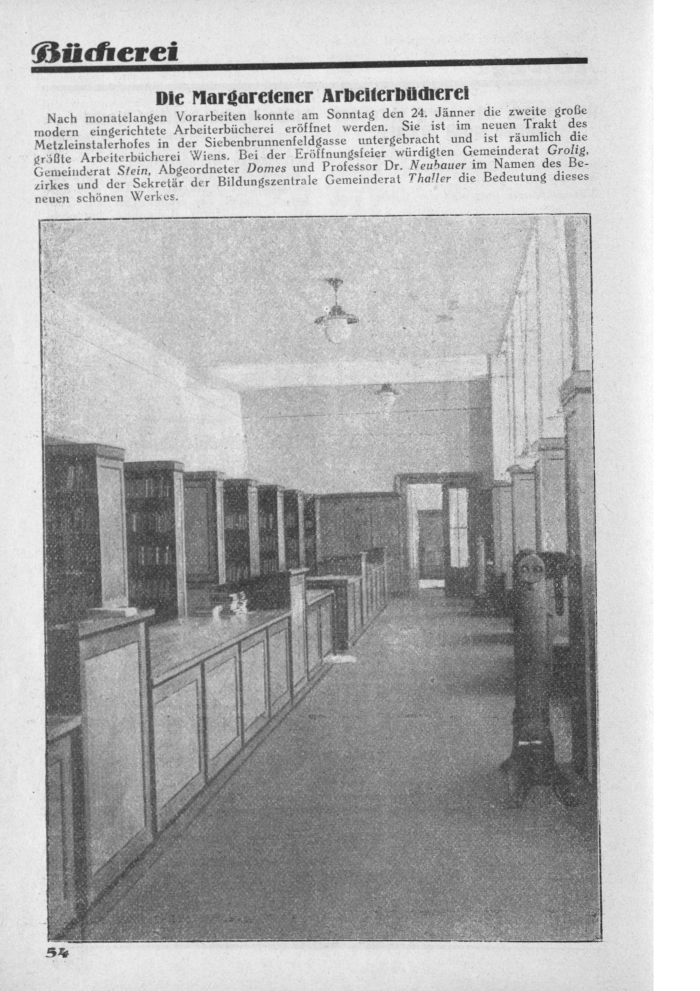
\includegraphics[width=.9\textwidth]{img/Schuldt01.jpg}
\caption{Blick in die 1926 eröffnete \enquote{Margaretener
Arbeiterbücherei}, Wien (in: Bildungsarbeit. Blätter für sozialistisches
Bildungswesen, XIII (1926) 3, 54 (Digitalisat der Österreichischen
Nationalbibliothek)}
\end{figure}

\begin{figure}
\centering
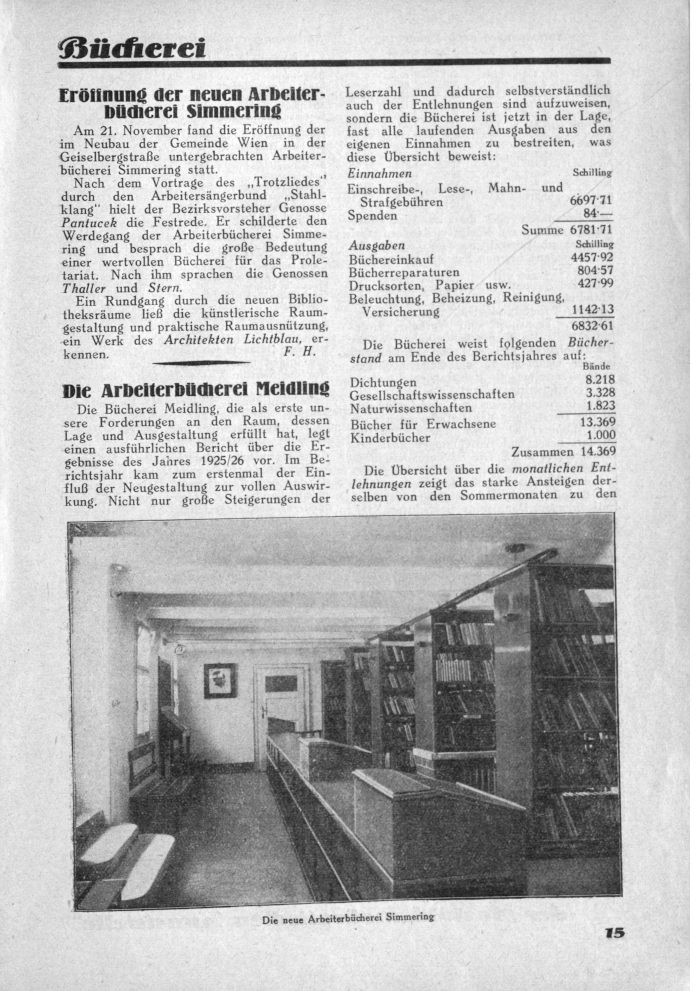
\includegraphics[width=.9\textwidth]{img/Schuldt02.jpg}
\caption{Blick in die \enquote{Arbeiterbücherei Simmering}, Wien (in:
Bildungsarbeit. Blätter für sozialistisches Bildungswesen, XIV (1927) 1,
15 (Digitalisat der Österreichischen Nationalbibliothek)}
\end{figure}

\hypertarget{der-bestand-kein-schmutz-kein-schund-fuxfcr-die-selbstbefreiung-des-proletariats}{%
\subsection{Der Bestand: Kein Schmutz, kein Schund -- für die
Selbstbefreiung des
Proletariats}\label{der-bestand-kein-schmutz-kein-schund-fuxfcr-die-selbstbefreiung-des-proletariats}}

Zum Bestand der \enquote{Arbeiterbibliotheken} fallen im Rückblick von
heute zwei Dinge auf: Die Sorge um die literarische Qualität und die
Fokussierung darauf, dass sich Arbeiterinnen und Arbeiter mit dem
Bestand selber bilden können sollten, um an der zukünftigen Gesellschaft
mitzuarbeiten.

Die Sorge um die Qualität teilten die \enquote{Arbeiterbibliotheken} mit
anderen Bibliothekstypen, allerdings mit einigen ideologischen
Besonderheiten. Qualität hiess hier, dass auch in
\enquote{Arbeiterbibliotheken} die Überzeugung vorherrschte, dass es (a)
Literatur von unterschiedlicher inhaltlicher, sprachlicher und
literarisch-künstlerischer Qualität gäbe, (b) dass diese Qualität einen
direkten Einfluss darauf hätte, wie sie bei den Leserinnen und Lesern
wirken würde -- sowohl als potentieller geistiger Aufstieg oder aber als
Gefahr für Denken, Moral und Verhalten --, ein Einfluss, welcher zudem
von den Bibliothekaren erkannt werden könnte und (c) dass es die Aufgabe
der Bibliothek wäre, den Lesenden beim potentiellen geistigen Aufstieg
durch das Lesen zu unterstützen. Damit verbunden waren Theorien über das
richtige Lesen, inklusive der Vorstellung, dass man sich als Leserin
oder Leser Qualitätsstufen hinaufbewegen müsse und dass deshalb Texte,
die man noch nicht erfassen könnte, weil sie zu komplex oder zu
qualitätsvoll wären, sich auch negativ auswirken würden. Was heute unter
dem Begriff der \enquote{Schmutz und Schund}-Debatte eher kurios klingt,
war damals eine weithin geteilte Überzeugung.

Die konkreten Ausformungen dieser Überzeugungen sind hier nicht Thema.
Wichtig ist die Grundstruktur, die von einer praktisch direkten Wirkung
von Literatur auf die Leserinnen und Leser sowie einer Gefährdung derer
Geisteskraft ausging und gleichzeitig reine Unterhaltungsfunktionen von
Literatur eher nicht anerkannte -- und der Fakt, dass sich in dieser
Überzeugung die \enquote{Arbeiterbibliotheken} mit der
Bücherhallenbewegung, dem katholischen Büchereiwesen oder auch der
\enquote{Volksbildungsbewegung} einig waren.

Wieder in der Broschüre von Gustav Hennig (Hennig 1908) finden sich
deshalb auch Statistiken der ausgeliehenen Bücher in der von im
betreuten Bibliothek. Es ging ihm um die konkreten Titel. Als
erfolgreich galt Bibliotheksarbeit, wenn nicht möglichst viele, sondern
möglichst die richtigen Bücher verliehen wurden, weil dies die
literarische Reife ihrer Leserinnen und Leser nachwies.

\begin{figure}
\centering
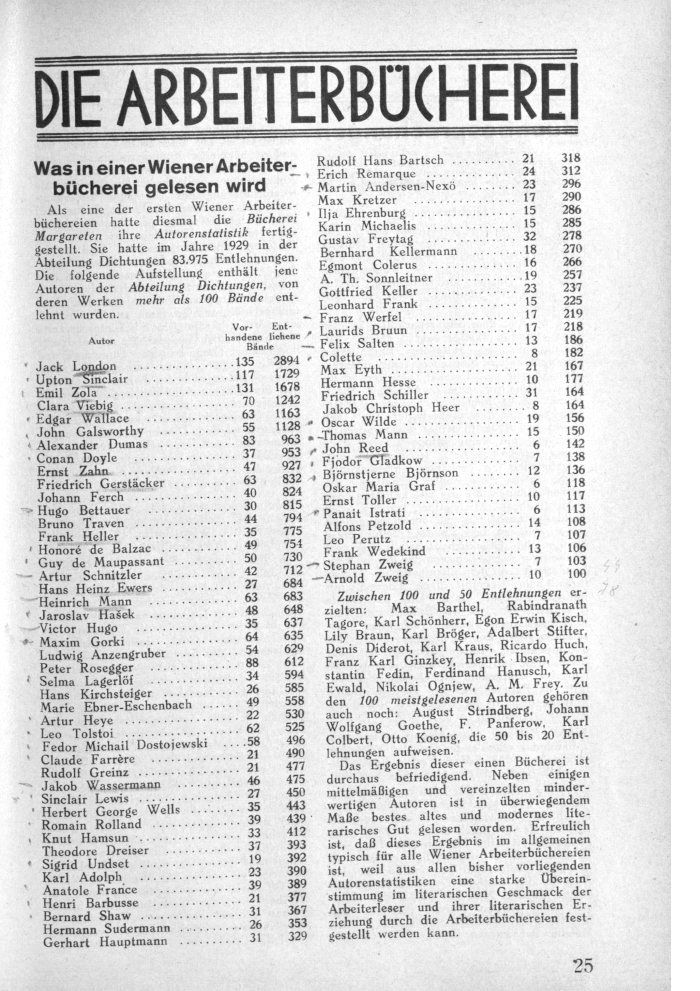
\includegraphics[width=.9\textwidth]{img/Schuldt03.jpg}
\caption{\enquote{Was in einer Wiener Arbeiterbibliothek gelesen wird},
eine (späte) Aufzählung der entliehenen Autorinnen und Autoren, die
zeigen sollte, dass qualitätsvolle Literatur gelesen wird. (in: Die
Arbeiterbücherei. Sonderbeilage zur: Bildungsarbeit. Blätter für
sozialistisches Bildungswesen, XVII (1930) (Digitalisat der
Österreichischen Nationalbibliothek)}
\end{figure}

\begin{figure}
\centering
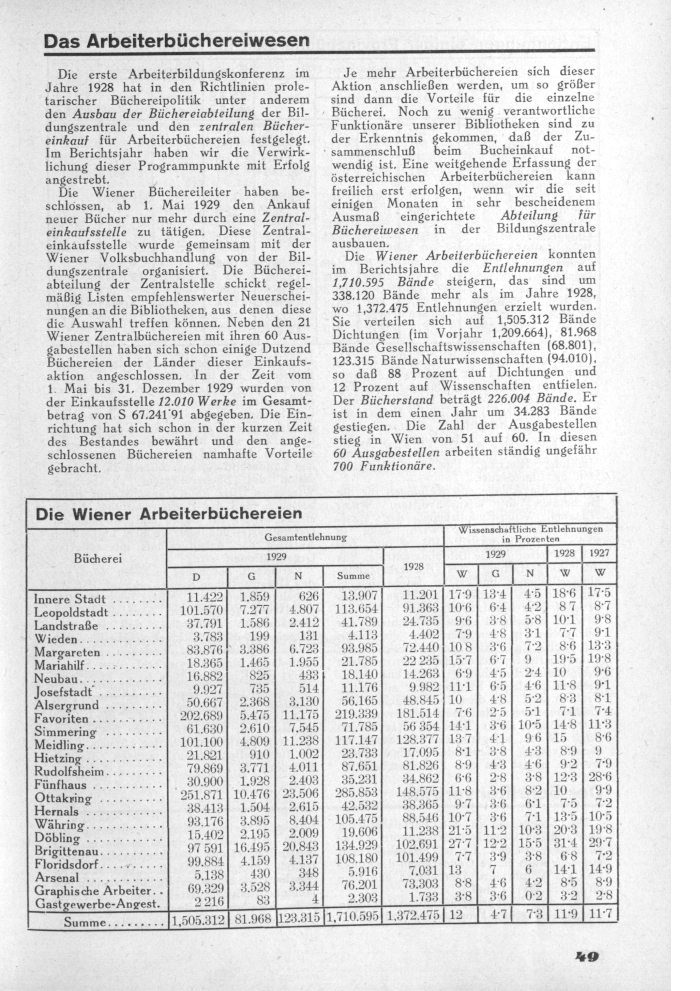
\includegraphics[width=.8\textwidth]{img/Schuldt04.jpg}
\caption{Jahresausleihstatistik der Wiener Arbeiterbüchereien 1929. Auch
hier wird Wert darauf gelegt zu zeigen, dass die Bibliotheken zur
wissenschaftlichen Bildung genutzt wurden und nicht nur zur
Unterhaltung. Legende: D - Dichtung (Belletristik), G -
Gesellschaftswissenschaften, N - Naturwissenschaften, W - Wissenschaft
insgesamt (in: Die Arbeiterbücherei. Sonderbeilage zur: Bildungsarbeit.
Blätter für sozialistisches Bildungswesen, XVII (1930) 4, 49
(Digitalisat der Österreichischen Nationalbibliothek)}
\end{figure}

Worin sich die \enquote{Arbeiterbibliotheken} unterschieden, war die
konkrete inhaltliche Bewertung. Es gab Literatur, die von
\enquote{Arbeiterbibliotheken} und Lesehallen zugleich als
\enquote{Schund} abgelehnt wurde. Aber daneben gab es Literatur, die der
Meinung der \enquote{Arbeiterbibliotheken} nach zur Aufrechterhaltung
der bestehenden Verhältnisse beitragen würde, in der die Arbeiterinnen
und Arbeiter zum Beispiel lernen würden, sich der Autorität von Staat,
Firmeneignern und Kirche unterzuordnen. Dies galt nicht nur für
explizite Propagandaschriften, sondern zum Beispiel auch für Literatur,
in der am Ende die Protagonistinnen und Protagonisten eine individuelle
Lösung im Glauben oder im kleinbürgerlichen Leben fanden. Das wurde
negativ gewertet. Literatur hingegen, welche das Leben der unteren
Sozialschichten darstellte, galt als positiv, weil sie die tatsächliche
Realität vermitteln würde. Bücher wurden nach solchen Kriterien
bewertet, diese auch gegeneinander abgewogen.

Mit dieser Eigenheit der Bestandsarbeit ging die zweite Besonderheit
einher: Die Bibliotheken sollten einerseits den Angehörigen der
\enquote{Arbeiterbewegung} Zugang zu Literatur ermöglichen, aber
andererseits auch das Ziel der Bewegung unterstützen, eine andere
Gesellschaft zu erreichen. Die Bibliotheken waren ein Bildungsmittel mit
einem klaren Ziel: Der Selbstbefreiung der Arbeiterinnen und Arbeiter
(und damit -- zumindest der meisten Vorstellungen nach, die in der
Arbeitervertretung verbreitet waren -- auch der Befreiung der restlichen
Welt). Die Leserinnen und Leser sollten die gesellschaftlichen und
historischen Zusammenhänge verstehen, inklusive ihrer Stellung in
diesen. Sie sollten sich bilden, um gesellschaftliche Funktionen
übernehmen zu können. Gleichzeitig sollten sie durch Bildung in
Betrieben aufsteigen -- als Teil gewerkschaftlicher Entwicklung. Das
konnte mit individuellem Aufstieg einhergehen, war aber gedacht als
Bildungsaufstieg der gesamten \enquote{Arbeiterbewegung}. Das
Bildungsziel war die Vorbereitung auf den Sozialismus und gleichzeitig
die bessere Vertretung der Interessen der Arbeitenden in der aktuellen
Gesellschaft.

Dieses Bildungsziel beeinflusste die Auswahl des Bestandes (und die
Beratung am Tresen) direkt. \enquote{Arbeiterbibliotheken} -- wie damals
auch andere Bibliotheken für breite Massen -- hatten normalerweise einen
Bestand von einigen Hundert bis zu wenigen Tausend Titeln. Insoweit war
im Bestand kein Platz vorhanden für Medien, die als politisch falsch
oder schwierig angesehen wurden. Jede Publikation des organisierten
Katholizismus oder der liberalen Bewegung hätte wohl eine Publikation
der \enquote{Arbeiterbewegung} weniger bedeutet. Als zu komplex
angesehen Publikationen, für welche die Arbeiterinnen und Arbeiter mit
den damaligen Arbeitsstunden keine Zeit hätten, um sie durchzuarbeiten,
galten ebenso als nicht notwendig. Eingestellt in den Bestand wurden
aber gerade nicht nur politische Schriften, sondern auch
populärwissenschaftliche Darstellungen und Literatur zu technischen,
soziologischen und naturwissenschaftlichen Themen, zur Weltliteratur und
Ähnlichem. In der zeitgenössischen Fachliteratur finden sich immer
wieder Abwägungen dazu: Wie verständlich sind bestimmte Werke? Wie sehr
beeinflusste die politische Haltung der Autorinnen und Autoren das Werk?
War der Inhalt für die sozialistische Bewegung vielleicht trotzdem
sinnvoll, obwohl die politische Haltung falsch war? Dabei wurde nicht
von einer Neutralität der politischen Anschauungen ausgegangen -- alle
Autorinnen und Autoren hätten eine Ideologie, die sie mit in ihre Werke
bringen würden. Aber es gäbe zum Beispiel Naturgesetze und Fakten, die
immer gleich wären.\footnote{Eine Haltung, die heute kritisiert werden
  kann. Auch Fakten sind sozial konstruiert, reproduziert und
  verhandelt. Aber eine solche Kritik an der Haltung der
  \enquote{Arbeiterbewegung} wäre anachronistisch.}

Die gleichen Fragen galten für Unterhaltung oder Kultur. Einerseits gab
es in der \enquote{Arbeiterbewegung} intensive Versuche, eine eigene
\enquote{proletarische Kultur} zu etablieren -- was auch unterschiedlich
aussehen konnte, sich aber zum Beispiel im \enquote{Roten Wien} der
1920er Jahre in Massenveranstaltungen für \enquote{Arbeitersport},
\enquote{Arbeitersingen} et cetera manifestierte --, die sich von der
restlichen Kultur, in der falsche Ideale und Ideologien vertreten
würden, unterscheiden sollte. Und gleichzeitig wurde versucht, die
besten \enquote{überzeitlichen} Werke der Welt- und Nationalliteraturen
zu integrieren. Deshalb gab es immer Werke, die nicht in
\enquote{Arbeiterbibliotheken} standen, dafür aber in Lesehallen und
katholischen Bibliotheken -- und andersherum. Gleichzeitig gab es Werke,
die in allen standen oder in keinen. Es ging nicht nur um die Frage der
literarischen Qualität, sondern auch um den konkreten Inhalt -- nicht
nur um \enquote{Schmutz und Schund}, sondern auch um Ideologie.

\hypertarget{kritik-am-buxfcrgerlichen-buxfcchereiwesen-neutralituxe4t-als-ideologie}{%
\section{\texorpdfstring{Kritik am \enquote{bürgerlichen
Büchereiwesen}: Neutralität als
Ideologie}{Kritik am \enquote{bürgerlichen Büchereiwesen}: Neutralität als Ideologie}}\label{kritik-am-buxfcrgerlichen-buxfcchereiwesen-neutralituxe4t-als-ideologie}}

In der \enquote{Arbeiterbewegung} wurde, wie gesagt, davon ausgegangen,
dass es (a) einen zentralen Antagonismus zwischen verschiedenen Klassen
gäbe, welcher (b) der Gesellschaft inhärent wäre, der (c) ökonomisch
begründet sein und (d) deshalb auch nicht verschwinden würde, solange
die Ökonomie so organisiert sei, wie sie sei -- also mit denen, die die
Produktionsmittel besitzen, von ihnen profitierten und deshalb
tendenziell ein Interesse daran hätten, dass diese ökonomischen
Strukturen aufrechterhalten bleiben und denen, die kein Eigentum dieser
Art hätten, aber gezwungen seien, mit diesen Produktionsmitteln zu
schaffen und die deshalb ein Interesse an der Veränderung dieser
Strukturen hätten. Um diesen Antagonismus herum -- der nicht ohne Grund
angenommen wurde -- organisierte sich die \enquote{Arbeiterbewegung},
interpretierte aber auch die gesamte Gesellschaft: Die Institutionen und
Infrastrukturen der \enquote{Arbeiterbewegung} hatten in dieser
Weltsicht die Aufgabe, die Ziele der eigenen Bewegung zu unterstützen.

Aus diesem Denken heraus war es folgerichtig, dass auch alle anderen
Institutionen und Infrastrukturen daraufhin befragt wurden, zu welchem
Ziel und mit welchen Vorstellungen sie eingerichtet und unterhalten
würden. Diese Weltsicht hatte ihre eigene inhaltliche Folgerichtigkeit
und wurde untermauert dadurch, dass es tatsächlich Institutionen,
Vereine, Unternehmungen anderer politischer Bewegungen gab, die jeweils
die Ziele dieser Bewegungen unterstützten. Aus dem Denken der
\enquote{Arbeiterbewegung} heraus galt dies für alle Einrichtungen, auch
wenn bei einigen genauer zu fragen war, wie und wozu sie wirkten.
Beispielsweise soziale Einrichtungen, die von Fabrikanten finanziert
wurden und bei denen sich die Frage stellte, wozu sie das taten: Damit
es den Arbeiterinnen und Arbeitern wirklich besser ginge oder damit sie
sich so verhielten, wie es in der Weltsicht der Finanziers vorgesehen
war? Wurden sie zum Beispiel besser behandelt als in anderen Fabriken,
aber gerade dadurch abgehalten sich selber zu organisieren? Und wenn ja,
war das so gewollt? Während heute vor allem Siedlungen, die von Fabriken
für ihre Arbeiterinnen und Arbeiter errichtet wurden -- in oft höherer
Bau- und Wohnqualität als in anderen Wohngegenden --, bekannt sind, gab
es solche Unternehmungen auch im Bibliotheksbereich: Gerade die
\enquote{Bücherhallenbewegung}, welche zur Zeit der
\enquote{Arbeiterbibliotheken} antrat, wieder einmal einen neuen Typ
Öffentlicher Bibliotheken zu etablieren, wurde unter diesem
Gesichtspunkt analysiert.

Die \enquote{Lesehallenbewegung} postulierte, dass die sich damals
entwickelnde moderne Gesellschaft einen neuen Typus von Öffentlichen
Bibliotheken benötigen würde. Als Vorbild wurden Public Libraries in den
USA angegeben. Diese neuen Lesehallen sollten sich auszeichnen durch:

\begin{enumerate}
\def\labelenumi{(\arabic{enumi})}
\item
  Einen demokratischen Zugang in dem Sinne, dass sie für alle Schichten
  offen ständen und sich auch um alle bemühten -- was dazu führte, dass
  man sich über die Interessen, Voraussetzungen und Lebensumstände von
  Menschen in unterschiedlichen sozialen Schichten Gedanken machte und
  zum Beispiel begann, unter diesen Befragungen über Leseverhalten und
  Leseinteressen durchzuführen.
\item
  Dem Verfolgen von Bildungszielen, die sich einerseits an die
  \enquote{Volksbildungsbewegung} anlehnten -- also dem gleichen Diskurs
  um literarische Qualität, der angeblichen Gefahr \enquote{schlechter
  Literatur} und der Notwendigkeit der Lenkung beziehungsweise Beratung
  der Leserinnen und Leser folgte, wie die
  \enquote{Arbeiterbibliotheken} -- und andererseits der individuellen
  Fort- und Weiterbildung für den Beruf -- als Förderung aller
  Potentiale der Bevölkerung -- dienen sollte.
\item
  Dabei jeweils die Nutzung der modernsten Formen der
  \enquote{Bibliothekstechnik} -- als Oberbegriff für die Organisation
  bibliothekarischer Arbeiten und gleichzeitig für technische
  Hilfsmittel -- um möglichst viele Leserinnen und Leser zu bedienen und
  zu beraten sowie möglichst schnell die richtigen Bücher an die
  richtigen Personen verleihen zu können -- was zu vielen
  bibliothekstechnischen Experimenten führte.
\item
  Die Ausstattung der Bibliotheken mit den Lesesälen, welche der
  Bewegung ihren Namen gaben. Diese Säle, in welchen sich Leserinnen und
  Leser direkt aufhalten, lesen und schreiben konnten, waren zuvor nicht
  normal in Bibliotheken für breite Massen.
\end{enumerate}

Mit der Lesehallenbewegung wurden sie immer mehr zum Normalfall. Neue
oder umgestaltete Bibliotheken erhielten mit der Zeit solche Säle, in
den publizierten Bauplänen tauchten sie auf, in der Fachliteratur
begannen Diskussionen, die nur durch das Vorhandensein dieser Säle
möglich und notwendig wurden, beispielsweise ob und wenn ja, welche
Zeitungen und Zeitschriften in ihnen ausliegen oder ob
Schreibmaterialien und Schreibmaschinen zur Verfügung gestellt werden
sollten.

Es gab verschiedene Kritik an den dann tatsächlich eingerichteten
Lesehallen, insbesondere, dass sie zu sehr auf bibliothekstechnische
Fragen fokussieren würden und damit zu wenig auf die notwendige Beratung
der Leserinnen und Leser. Ausserdem wurde bezweifelt, das sie überhaupt
einen qualitativ hochwertigen Bestand aufbauen könnten, wenn sie sich an
den Interessen der Leserinnen und Leser orientieren. Und dennoch hatten
sie einen merklichen Einfluss. Auch die \enquote{Arbeiterbibliotheken}
wurden nach und nach mit Lesesälen ausgestattet; bibliothekstechnische
Neuerungen wurden ebenso übernommen oder selber entwickelt.

Gleichwohl waren die Lesehallen abhängig davon, dass sie finanziert
würden. Auch sie wollten einen kostenfreien Zugang bieten. Die
\enquote{Arbeiterbibliotheken} wurden, wie dargestellt, von der
\enquote{Arbeiterbewegung} getragen. Die Lesehallen hingegen wurden
hauptsächlich aus zwei Quellen finanziert: von philanthropischen
Firmeneignern und von Gemeinden (die bis 1918 nicht von Parteien der
\enquote{Arbeiterbewegung} regiert wurden). Für die Lesehallen war
gerade die kommunale Finanzierung die anzustrebende, ideale Lösung. Sie
verstanden sich als Institutionen für die gesamte Bevölkerung, die in
einer modernen Gesellschaft von den Kommunen getragen werden müssten, so
wie andere öffentliche Einrichtungen für die gesamte Bevölkerung auch.

Eine Kritik aus den \enquote{Arbeiterbibliotheken} setzte hier an: Wenn
die Gesellschaft aus Gruppen gebildet würde, die letztlich
antagonistische Interessen hätten, wie könnte es dann Institutionen
geben, die nicht von diesen Interessen geprägt seien? Genauso wie die
\enquote{Arbeiterbibliotheken} Teil der \enquote{Arbeiterbewegung} waren
und damit eine Ideologie vertraten und letztlich das Ziel unterstützten,
eine andere Gesellschaft zu schaffen, war zu vermuten, dass auch
Lesehallen und andere öffentliche Büchereien eine Ideologie vertraten
und ein Ziel unterstützten, selbst wenn sie einen anderen Anspruch
vertraten. Bei den Bibliotheken, die vom politisch organisierten
Katholizismus unterhalten wurden, war dies einfach zu sehen: Sie sollten
die Gesellschaft nach dem Bild dieser politischen Richtung umformen
respektive aufrecht erhalten.

Lesehallen und andere öffentliche Büchereien verstanden sich aber selber
nicht als solche politischen Einrichtungen. Vielmehr gingen sie davon
aus, für die gesamte Bevölkerung zu agieren. Die folgerichtige Vermutung
war allerdings, dass sie dennoch eine Ideologie, also eine Weltsicht
vertraten und versuchten, diese in die Realität umzusetzen. Wie sah
diese Ideologie dann aus, welche aus Sicht der
\enquote{Arbeiterbewegung} den Lesehallen vorgeworfen (oder
nachgewiesen) werden konnte?

\begin{enumerate}
\def\labelenumi{(\arabic{enumi})}
\item
  Der Antagonismus, welcher für das Denken der
  \enquote{Arbeiterbewegung} zentral war, würde zwar nicht per se
  bestritten -- auch die Bücherhallenbewegung ging explizit von
  unterschiedlichen sozialen Schichten aus --, aber seine Bedeutung
  wurde gänzlich anders eingeschätzt: (a) Dass die ökonomische Struktur
  diese Schichten hervorbrächte, sei natürlich und kein grundsätzliches
  Problem, welches überwunden werden müsse. (b) Der Wechsel zwischen den
  Schichten sei durch Bildung möglich; wichtig sei, dass Menschen Zugang
  zu Bildung hätten, dann würden die Tüchtigsten der unteren Schichten
  aufsteigen können. (c) Es gäbe übergreifende Interessen, welche für
  die ganze Bevölkerung gelten würden. Jede politische Bewegung würde
  dagegen Partikularinteressen vertreten. (d) Die Welt sei nicht anhand
  der ökonomischen Verhältnisse und Strukturen geteilt, sondern anhand
  anderer Strukturen (zum Beispiel Nationen, Kulturen,
  \enquote{Rassen}).
\item
  Hieraus ergäbe sich, dass man durch Bildung und Kultur die
  unterschiedlichen sozialen Voraussetzungen ausgleichen könnte, also
  zum Beispiel durch Lesehallen auch Arbeiterinnen und Arbeitern eine
  Möglichkeit bieten, welche Personen in anderen Schichten schon durch
  ihre Herkunft hätten. Die Verantwortung, diese Möglichkeiten zu
  nutzen, läge dann bei den Einzelnen. Es gäbe ein gemeinsames Interesse
  aller, diese Möglichkeiten zu schaffen. Alle würden davon profitieren,
  wenn die Besten einer Schicht aufstiegen.
\item
  Aus diesen gemeinsamen Interessen und dem Fakt, dass die ökonomische
  Struktur der Gesellschaft nicht der prägende Teil sei, welcher das
  Leben in der Gesellschaft bestimme, ergäbe sich auch, dass es Werte
  gäbe, die für alle bestimmend wären, beispielsweise was gute Literatur
  sei und was nicht.
\item
  Die Grundstruktur der Gesellschaft sei nicht zu verändern
  beziehungsweise sei die Frage, ob dies möglich wäre, für die
  Lesehallen irrelevant. Gewendet als Kritik hiess dies, dass die
  Lesehallen vor allem die Reproduktion und Aufrechterhaltung der
  existierenden Verhältnisse, wenn auch nicht unbedingt anstreben, so
  doch betreiben würden. Wenn zum Beispiel die Idee vertreten wird, dass
  die, die sich anstrengen würden, in der Gesellschaft aufsteigen
  könnten -- so es nur die Möglichkeit zur Bildung gibt --, dann würde
  die Frage irrelevant, warum es überhaupt diese Unterschiede zwischen
  den sozialen Schichten gibt. Und damit würden diese gesellschaftlichen
  Strukturen als normal akzeptiert.
\item
  Daraus ergäbe sich auch, dass der Anspruch der Lesehallen, die
  Literatur gleichsam neutral auszuwählen und bei der Beratung am Tresen
  neutral zu vermitteln, immer nur individuell gedacht würde, aufbauend
  auf den angenommen Fähigkeiten und Interessen der individuellen
  Leserinnen und Leser, aber ohne ein Interesse daran, wie diese
  Fähigkeiten und Interessen über den individuellen Fall hinaus konkret
  entstanden sind. Letztlich wäre das Ziel der Lesehallen, die
  existierenden gesellschaftlichen Strukturen zu erhalten und unter
  anderem Arbeiterinnen und Arbeiter davon abzuhalten, zu verstehen, wie
  die Gesellschaft strukturiert und wie diese Struktur zu überwinden
  sei.
\end{enumerate}

Die angebliche Neutralität sei gar keine -- und könne es auch gar nicht
sein. Jede Einrichtung hätte eine Aufgabe im Bezug darauf, die
Gesellschaft, wie sie ist, zu erhalten oder zu verändern. Die hinter den
Lesehallen stehende Vorstellung, man könne ausserhalb dieser Fragen
stehen, sei falsch -- und zwar aufgrund eines falschen Verständnisses
davon, wie diese Gesellschaft funktioniere.

Ausgehend von dieser Analyse wurde die Finanzierung der Lesehallen durch
Unternehmen und Kommunen interpretiert als ein Mittel, die Strukturen
der Gesellschaft zu erhalten. Am Ende lief diese Kritik darauf hinaus,
dass die Lesehallen vor allem deshalb finanziert wurden, weil die
Schichten, die von den gesellschaftlichen Strukturen profitierten -- in
der Diktion der \enquote{Arbeiterbewegung}: die herrschenden Klassen
beziehungsweise die Bourgeoisie --, auch von der Existenz dieser
Einrichtungen profitierten.

Diese Kritik an Lesehallen schloss, wie gesagt, nicht aus, dass
\enquote{Arbeiterbibliotheken} an den gleichen bibliothekstechnischen
Entwicklungen interessiert waren wie die Lesehallen oder inhaltliche
Vorstellungen in Bezug auf Literatur und literarische Qualität teilten.

\hypertarget{das-ende-der-arbeiterbibliotheken}{%
\section{\texorpdfstring{Das Ende der
\enquote{Arbeiterbibliotheken}}{Das Ende der \enquote{Arbeiterbibliotheken}}}\label{das-ende-der-arbeiterbibliotheken}}

Um die Bedeutung der damaligen Kritik für die heutige Zeit
einzuschätzen, ist es notwendig, kurz zu referieren, warum es heute
keine \enquote{Arbeiterbibliotheken} mehr gibt. Sind sie vielleicht
verschwunden, weil ihre eigene Weltsicht -- und damit ihre Kritik an den
Lesehallen aus dieser Weltsicht heraus -- falsch war?

Das scheint nicht so.

Was die \enquote{Arbeiterbibliotheken} zu einem Ende brachte, war das
Ende der \enquote{Arbeiterbewegung} und die wirtschaftliche Krise nach
dem Ersten Weltkrieg. Die \enquote{Arbeiterbibliotheken} in Sachsen und
Thüringen, welche von Gustav Hennig geprägt wurden, verschwanden in den
1920er Jahren nach und nach. (Marwinski 1994) Die Parteien der
\enquote{Arbeiterbewegung} (allen voran die SPD) übernahmen in mehr und
mehr Gemeinden die politische Macht und überführten
\enquote{Arbeiterbibliotheken} in kommunale Strukturen. Auch das war
folgerichtig: Wenn die \enquote{Arbeiterbewegung} die politische Macht
übernähme -- so wie zuvor die \enquote{herrschenden Klassen} die
politische Macht hatten -- und somit auf dem Weg zum Sozialismus sei,
dann würden diese -- also kommunale Struktur und
\enquote{Arbeiterbewegung} -- zusammenfallen. (Dass dies nicht so
eintrat, dass also die sozialistische Gesellschaft nicht geschaffen
wurde, schien Anfang der 1920er Jahre nicht ausgemacht.) Gleichzeitig
geriet die \enquote{Arbeiterbewegung}, die ja hauptsächlich von
Arbeitenden finanziert wurde, mit der Wirtschaftskrise Anfang der 1920er
Jahre in finanzielle Schwierigkeiten. Partei- und Gewerkschaftsbeiträge
sowie Spenden gingen zurück, zudem splitterte sich die Bewegung weiter
auf. Einrichtungen der \enquote{Arbeiterbewegung}, wie auch die
\enquote{Arbeiterbibliotheken}, wurden geschlossen, weil sie nicht mehr
finanziert werden konnten.

Auch die recht gut dokumentierte \enquote{Heimannsche Bibliothek}
schloss wegen finanzieller Probleme. (Strocher 1987) Sie war 1899 vom
sozialdemokratischen Reichstagsabgeordneten Hugo Heimann begründet
worden. Dieser hatte eine grössere Buchhandlung geerbt, verkauft und vom
Gewinn eine Einrichtung geschaffen, die Vorbildcharakter hatte: in einem
Arbeiterquartier in Berlin-Kreuzberg gelegen, mit grossem Lesesaal,
Freihandbestand in diesem Saal, mehr frei ausliegenden Zeitschriften als
in den kommunalen Büchereien, mit fest angestelltem Personal
ausgestattet und frei zugänglich. Lange galt sie als Vorzeigeeinrichtung
der \enquote{Arbeiterbewegung} -- als Beweis dafür, was möglich wäre,
wenn man nur wollte. Auch diese Bibliothek, die praktisch von der
\enquote{Arbeiterbewegung} und Spenden finanziert wurde, schloss 1919
und wurde 1920 in das kommunale Büchereiwesen überführt.

Zum System der \enquote{Arbeiterbibliotheken} in Wien ist ebenso relativ
viel bekannt. (Pfoser 1980) In Wien dominierte -- im Gegensatz zum
restlichen Österreich -- von 1918 bis 1934 die heutige SPÖ. Sie
dominierte auch die \enquote{Arbeiterbewegung} weit mehr, als das der
SPD in Deutschland gelang. Diese Jahre des \enquote{Roten Wien} waren
geprägt durch einen Ausbau der öffentlichen Infrastruktur unter sozialen
Gesichtspunkten: Die städtischen Wohnungen wurden massiv vermehrt,
Schulen, Krankenhäuser, der ÖPNV relevant ausgebaut. Die
\enquote{Arbeiterbibliotheken} wurden allerdings gerade nicht in die
kommunale Verwaltung überführt. Vielmehr wurden diese -- neben den
kommunalen Büchereien -- gezielt ausgebaut als Teil des Aufbaus einer
umfassenden Infrastruktur der SPÖ für eine eigenständige
\enquote{Arbeiterkultur} mit Zeitschriften, Verlagen, Theater- und
Singvereinen, die immer dort stark waren, wo die SPÖ stark war. Die
\enquote{Arbeiterbibliotheken} in Wien stellten ein umfassendes Netz
dar: Tresenbibliotheken, Lesehallen, Kinderlesehallen, vertreten in
jedem Wiener Bezirk, teilweise mehrfach und getragen von der
\enquote{Arbeiterbewegung} selbst, sowohl finanziell als auch vom -- oft
ehrenamtlichen -- Personal her. Auch diese Arbeiterkulturbewegung sollte
die zukünftige Gesellschaft vorbereiten und erreichen helfen. Die Wiener
\enquote{Arbeiterbibliotheken} wurden in der Presse der SPÖ gerne als
Errungenschaften vorgeführt.

Ein Ende wurden diesen \enquote{Arbeiterbibliotheken} erst durch den
Ständestaat -- also der Diktatur der \enquote{Vaterländischen Front}
unter Dollfuß und Schussnig -- und dem darauffolgenden
Nationalsozialismus gemacht. Nach der Übernahme der Macht im
Österreichischen Bürgerkrieg 1934 wurde der SPÖ-Bürgermeister von Wien
abgesetzt und im Laufe der nächsten Jahre (unter anderem) die
\enquote{Arbeiterbibliotheken} mit den kommunalen Büchereien
zusammengelegt, dabei dann auch ihre Struktur und ihr Inhalt verändert.

\begin{figure}
\centering
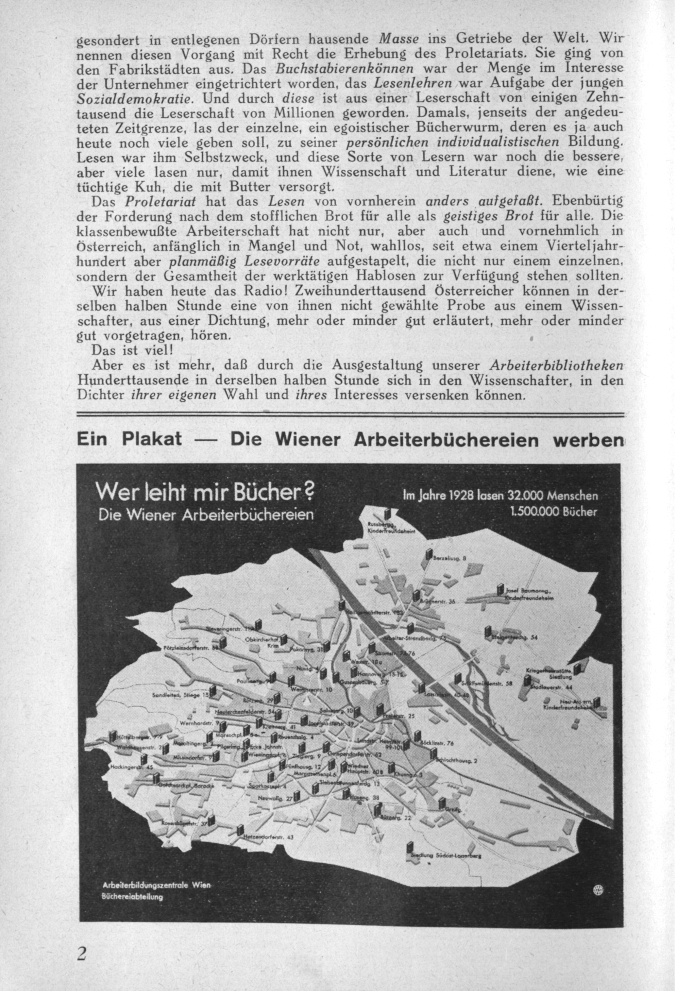
\includegraphics[width=.9\textwidth]{img/Schuldt05.jpg}
\caption{Plakat mit allen Wiener Arbeiterbüchereien 1928, auf dem
Höhepunkt ihrer Aktivitäten. (in: Die Arbeiterbücherei. Sonderbeilage 1
zur: Bildungsarbeit. Blätter für sozialistisches Bildungswesen, XVII
(1930) (Digitalisat der Österreichischen Nationalbibliothek)}
\end{figure}

\begin{figure}
\centering
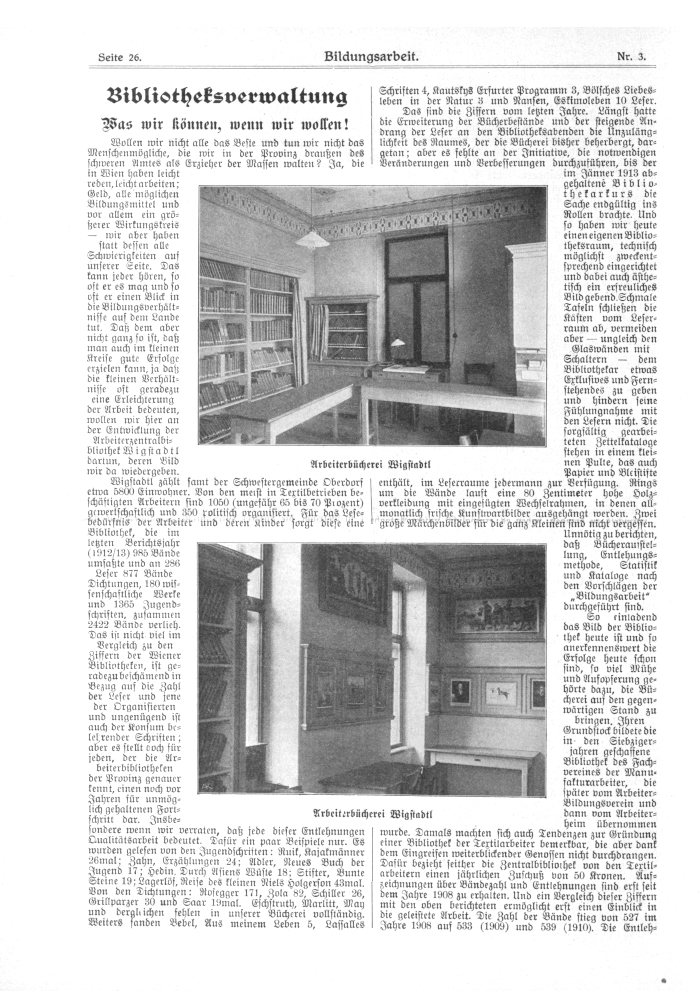
\includegraphics[width=.8\textwidth]{img/Schuldt06.jpg}
\caption{Hans Honheiser: \enquote{Bibliotheksverwaltung: Was wir können,
wenn wir wollen}. Der Titel des Beitrags eines Arbeiterbibliothekars aus
Wien zeigt, wie die Bibliotheken als Beispiel dafür angeführt werden,
dass die \enquote{Arbeiterbewegung} zur Organisation aller möglichen
Einrichtungen fähig wäre. Interessant auch die Bilder aus der kleineren
Arbeiterbibliothek des Autors. Auch diese funktioniert als
Thekenbibliothek. (in: Die Arbeiterbücherei. Sonderbeilage 3 zur:
Bildungsarbeit. Blätter für sozialistisches Bildungswesen, XVII (1930)
26--27 (Digitalisat der Österreichischen Nationalbibliothek)}
\end{figure}

Insoweit kann man sagen, dass die \enquote{Arbeiterbibliotheken} nicht
an sich selber gescheitert sind und auch nicht daran, dass zu wenig
Interesse an ihrer Nutzung bestanden hätte, sondern an Umständen
ausserhalb ihrer selbst. Allerdings solchen, die sie eigentlich hätten
verhindern helfen sollen.\footnote{Dazu passt, dass
  \enquote{Arbeiterbibliotheken} in der Schweiz offenbar über den
  Zweiten Weltkrieg hinaus existierten und ihre Spuren erst zur Zeit des
  Kalten Krieges verschwanden. (Siehe zum Beispiel Haag 1982.)}

Zu vermerken ist, dass nach dem Nationalsozialismus nicht mehr an die
\enquote{Arbeiterbibliotheken} angeschlossen wurde. Die SPÖ -- seit 1945
wieder die Politik in Wien dominierend -- führte stattdessen das
kommunale Bibliothekswesen weiter (und hat heute auch nicht mehr das
Ziel einer sozialistischen Gesellschaft). In der SBZ und später der DDR
wurde ebenfalls an die kommunalen Bibliotheken angeschlossen und neue
Bibliothekssysteme aufgebaut, wobei diese Bibliotheken -- wie andere
Bildungseinrichtungen auch -- politisch erst für den Aufbau, dann den
Erhalt der sozialistischen Gesellschaft, wie sie in der DDR verstanden
wurde, verpflichtet wurden. Erst in den 1980er Jahren scheint wieder ein
Interesse an den \enquote{Arbeiterbibliotheken} entstanden zu sein.
(Schumann \& Reinhardt 1984) Aber auch das gilt nicht nur für die
\enquote{Arbeiterbibliotheken} allein, sondern auch für andere
Bibliothekstypen. In diesem Text wurde mehrfach auf die Bibliotheken des
politisch organisierten Katholizismus verwiesen. Auch diese wurden nach
1945 in das Öffentliche Bibliothekswesen integriert, wenn auch oft in
kirchlicher Trägerschaft. Es gab aber Ende des 19. und Anfang des 20.
Jahrhunderts weit mehr Bibliothekstypen. Diese werden in der
Bibliotheksgeschichtsschreibung oft übergangen und dafür eine
historische Linie von den Lesehallen zu den heutigen Öffentlichen
Bibliotheken gezogen. Aber zumindest bis zu den 1920er Jahren war nicht
klar, welcher Bibliothekstyp sich durchsetzen würde. All diese
Bibliothekstypen, von denen einige -- wie die
\enquote{Arbeiterbibliotheken} -- über Jahrzehnte erfolgreich waren,
stellten Alternativentwürfe zu den Lesehallen dar (und vice versa),
deren Existenz allein immer eine implizite Kritik an den anderen
Bibliothekstypen vermittelte: So, wie ein spezifischer Bibliothekstyp
war, musste er nicht sein. Es ging immer auch anders.\footnote{Anzumerken
  ist, dass auch heute noch politische Bewegungen immer wieder
  Bibliotheken gründen, um die Ziele der eigenen Bewegung zu
  unterstützen. Beispielsweise tauchen in der Literatur der
  \enquote{Instandsbesetzungsbewegung} der 1980er Jahre immer wieder
  Bibliotheksprojekte auf. Die Bibliotheken, welche bei den
  Occupy-Protesten 2011--2012 eingerichtet wurden, sind ebenfalls immer
  wieder einmal Thema von Berichten geworden. Das Monopol der
  Öffentliche Bibliotheken ist auch heute nicht unumstritten. (Siehe
  dazu LIBREAS \#26.)}

\hypertarget{fazit-kann-die-uxf6ffentliche-bibliothek-eine-neutrale-bibliothek-sein}{%
\section{Fazit: Kann die Öffentliche Bibliothek eine neutrale
Bibliothek
sein?}\label{fazit-kann-die-uxf6ffentliche-bibliothek-eine-neutrale-bibliothek-sein}}

\enquote{Arbeiterbibliotheken} bestanden also über mehrere Jahrzehnte
als erfolgreicher Bibliothekstyp und übten unter anderem an einer
Bibliotheksform Kritik, die in vielem das vertrat, was heute im
Bibliothekswesen als Grundlage verstanden wird -- insbesondere der
Behauptung, auf weltanschauliche Neutralität verpflichtet zu sein.
Verstärkt wurde diese Kritik durch die praktische Existenz der
\enquote{Arbeiterbibliotheken} selber: Andere Formen von Bibliotheken
als die Lesehallen waren offenbar möglich.

Die Frage ist, ob die Kritik der \enquote{Arbeiterbibliotheken} an den
Lesehallen mit ihrer \enquote{bürgerlichen Bibliotheksideologie} auch
für die heutigen Öffentlichen Bibliotheken gilt. Diese Vermutung lässt
sich nicht so leicht zurückweisen.

\begin{enumerate}
\def\labelenumi{(\arabic{enumi})}
\item
  Die \enquote{Arbeiterbibliotheken} stellten aus ihrer Position als
  eindeutig politisch verortete Bibliotheken die Frage, ob es überhaupt
  möglich ist, eine \enquote{neutrale} Bibliothek einzurichten. Sie
  verneinten das. In einer Gesellschaft, die sich um einen ökonomischen
  Antagonismus herum organisiert, sei es unmöglich, nicht entweder zum
  Erhalt dieses Antagonismus beizutragen oder zu seiner Veränderung. Es
  gäbe keine Position ausserhalb dieses Antagonismus, selbst wenn
  behauptet würde, die eigene Bibliothek würde sich zu diesem neutral
  verhalten. Heute würde man die Gesellschaft anders begreifen und
  vielleicht mehr Widersprüche benennen. Wie kann man sich zum Beispiel
  in einer Gesellschaft, die Geschlechter binär reproduziert und
  Chancen, Einfluss, Möglichkeiten anhand dieser verteilt, ausserhalb
  dieser ständigen Reproduktion verorten? Wird man durch seine Arbeit
  als Bibliothek nicht immer zu dieser Reproduktion beitragen oder diese
  verändern? Aber die grundsätzliche Frage der
  \enquote{Arbeiterbibliotheken} -- kann eine Einrichtung in einer von
  strukturellen Widersprüchen geprägten Gesellschaft überhaupt neutral
  sein -- ist weiterhin offen.
\item
  Wieder aufgrund ihrer Position, Teil einer Bewegung mit einem
  expliziten politischen Ziel zu sein, vermuteten die
  \enquote{Arbeiterbibliotheken}, dass jede andere Einrichtung auch ein
  politisches Ziel unterstütze, selbst wenn sie sich das selbst nicht
  eingestehen würde. Die Lesehallen mit ihrem Anspruch, weltanschaulich
  neutral zu sein, würden stattdessen die Reproduktion der ökonomischen
  Verhältnisse unterstützen. (Und das sei falsch, weil diese
  Verhältnisse falsch seien.) Auch diese Frage ist weiterhin virulent.
  Zu welchem Zweck machen Öffentliche Bibliotheken eigentlich ihre
  Arbeit? Was ist ihr Ziel? Worauf diese Frage hindeutet, ist, dass
  Bibliotheken selber in der Lage sind, diese Ziele zu bestimmen und
  dass sie eben nicht von aussen bestimmt sind. Wenn Bibliotheken diese
  Ziele von aussen bestimmen lassen, würden sie tendenziell die
  bestehenden gesellschaftlichen Strukturen mitreproduzieren und
  unterstützen.
\item
  Die \enquote{Arbeiterbibliotheken} fragten auch, welches Bild von
  Gesellschaft und Individuen eigentlich hinter der konkreten
  Bibliotheksarbeit stand. Die Lesehallen würden die Gesellschaft so
  verstehen, als ob die wirtschaftliche und politische Ordnung
  tendenziell so sein müsse, wie sie ist und als wären vor allem die
  einzelnen Individuen in der Lage, durch eigene Anstrengungen
  aufzusteigen. Die \enquote{Arbeiterbibliotheken} hingegen würden eine
  andere Ideologie vertreten. Auch diese Frage ist aktuell geblieben,
  selbst wenn man diese nicht auf Basis einer ausformulierten Ideologie
  stellt, wie das die \enquote{Arbeiterbibliotheken} tun konnten. Was
  sie sichtbar machte und weiter sichtbar hält, ist, dass jede
  bibliothekarische Arbeit ihre Basis in einer Weltanschauung hat und
  dass es sich lohnt, nach dieser Weltanschauung zu fragen, insbesondere
  dann, wenn behauptet wird, Einrichtungen wie Bibliotheken würden
  neutral ausserhalb von Weltanschauungen stehen (können). Eine solche
  Behauptung, so kann man von den \enquote{Arbeiterbibliotheken} lernen,
  ist nicht per se überzeugend. Irrelevant scheint dabei, ob
  Bibliotheken den jeweils neuesten bibliothekstechnischen Entwicklungen
  folgen oder ob sie grosse Teil der Überzeugungen davon, was
  Bibliotheksarbeit ausmacht, teilen. Das hielt zumindest die
  \enquote{Arbeiterbibliotheken} auch nicht von ihrer Kritik zurück.
\end{enumerate}

\hypertarget{literatur}{%
\section*{Literatur}\label{literatur}}

\hypertarget{zeitschriften}{%
\subsection*{Zeitschriften}\label{zeitschriften}}

\emph{Bibliothekar und Ratgeber für Hausbüchereien : Monatsschrift für
Arbeiterbibliotheken}. (1918--1922) Gera

\emph{Der Bibliothekar. Monatsschrift für Arbeiterbibliotheken}.
(1907--1917) Leipzig

\emph{Bildungsarbeit. Blätter für Sozialistisches Bildungswesen}.
(1909--1914 und 1919--1934) Wien,
\url{http://anno.onb.ac.at/cgi-content/anno-plus?aid=bar}

\hypertarget{monografien}{%
\subsection*{Monografien}\label{monografien}}

Brünle, Elke. \emph{Bibliotheken von Arbeiterbildungsvereinen im
Königreich Württemberg : 1848--1918} (Mainzer Studien zur
Buchwissenschaft, 20). Wiesbaden: Harrassowitz, 2010

Haag, Verena. \emph{Die ehemalige Arbeiterbibliothek Aarau : Geschichte,
Umfeld, Teilintegration in die Aargauische Kantonsbibliothek}
(Diplomarbeit). Aarau : Aargauische Kantonsbibliothek, 1982

Heidenreich, Frank. \emph{Arbeiterkulturbewegung und Sozialdemokratie in
Sachsen vor 1933} (Demokratische Bewegungen in Mitteldeutschland, 3).
Weimar : Böhlau, 1995

Hennig, Gustav. \emph{Zehn Jahre Bibliothekarbeit : Geschichte einer
Arbeiterbibliothek : ein Wegweiser für Bibliothekverwaltungen}. Leipzig
: Verlag der Leipziger Buchdruckerei, 1908

Marwinski, Felicitas. \emph{Sozialdemokratie und Volksbildung : Leben
und Wirken Gustav Hennigs als Bibliothekar} (Beiträge zur
Bibliothekstheorie und Bibliotheksgeschichte, 9). München u.a.: K.G.
Saur Verlag, 1994

Pfoser, Alfred. \emph{Literatur und Austromarxismus}. Wien : Löcker
Verlag, 1980

Schroeder, Werner. \emph{"Arbeiter, fördert und unterstützt weiter eure
geistige Rüstkammer" : Aufbau, Bedeutung und Zerschlagung der
Arbeiterbibliotheken in Thüringen} (Veröffentlichungen der Bibliothek
der Friedrich-Ebert-Stiftung, 20). Bonn : Bibliothek der
Friedrich-Ebert-Stiftung, 2008

Schumann, Ilse; Reinhard, Gabriele. \emph{Über ehemalige
Arbeiterbibliotheken 1899 - 1933 im heutigen Bezirk Potsdam}
(Ausstellungsdokumentation). Potsdam: Wissenschaftliche
Allgemeinbibliothek des Bezirkes Potsdam, 1984

Strocher, Norbert. \emph{Die Heimannsche "Öffentliche Bibliothek und
Lesehalle zu unentgeltlicher Benutzung für jedermann" 1899-1919 : eine
Bibliothek für die Berliner Arbeiterschaft} (Beiträge zur Berliner
Bibliotheksgeschichte, 5). Berlin: Bibliotheksverband der Deutschen
Demokratischen Republik, Bezirksgruppe Berlin, 1987

Vodosek, Peter. \emph{Arbeiterbibliothek und öffentliche Bibliothek :
zur Geschichte ihrer Beziehungen von der ersten Hälfte des 19.
Jahrhunderts bis 1933} (Schriftenreihe der Bibliothekar-Lehrinstitut,
Reihe B: Dozentenschriften, 2). Berlin : Deutscher Bibliotheksverband,
1975

%autor
\begin{center}\rule{0.5\linewidth}{\linethickness}\end{center}

\textbf{Karsten Schuldt}, Dr., Wissenschaftlicher Mitarbeiter am
Schweizerischer Institut für Informationswissenschaft, HTW Chur.
Redakteur der LIBREAS. Library Ideas.

\end{document}
